\newpage
\subsection{Fonctionnalité 4}
La fonctionnalité 4 consiste en premier lieu à faciliter le remplissage du formulaire par l'établissement. 
Une complétion automatique du nom de la ville, de l'établissement, des niveaux scolaires devra être mise en place. Cependant, il n'y en aura pas pour les informations personnelles du demandeur (comme  par exemple son numéro de téléphone ou son adresse électronique).\\
La figure \ref{recevoirDemandesDIntervention} présentera un diagramme de cas d'utilisation présentant la réception de demande d'intervention d'un établissement.\\
Les données personnelles concernant les contacts dans l'établissement seront seulement un complément des informations disponibles pour un établissement. Elles pourront être mises à jour chaque année dans différents cas comme par exemple lors d'une mutation ou d'un départ en retraite ou encore d'un nouvel enseignant.   \\

La fonctionnalité 4 permettra également l'envoi d'un e-mail de confirmation à l'établissement lorsque ce dernier aura rempli et validé le formulaire. Cet e-mail proposera également à l'établissement d'annuler la demande d'intervention. \\ Une copie de cet e-mail sera adressée au responsable local de chaque activité.
La figure \ref{maquetteCourrielConfirmation} présentera une maquette de l'e-mail de confirmation de l'établissement.\\
\begin{figure}[H]
	\centering
	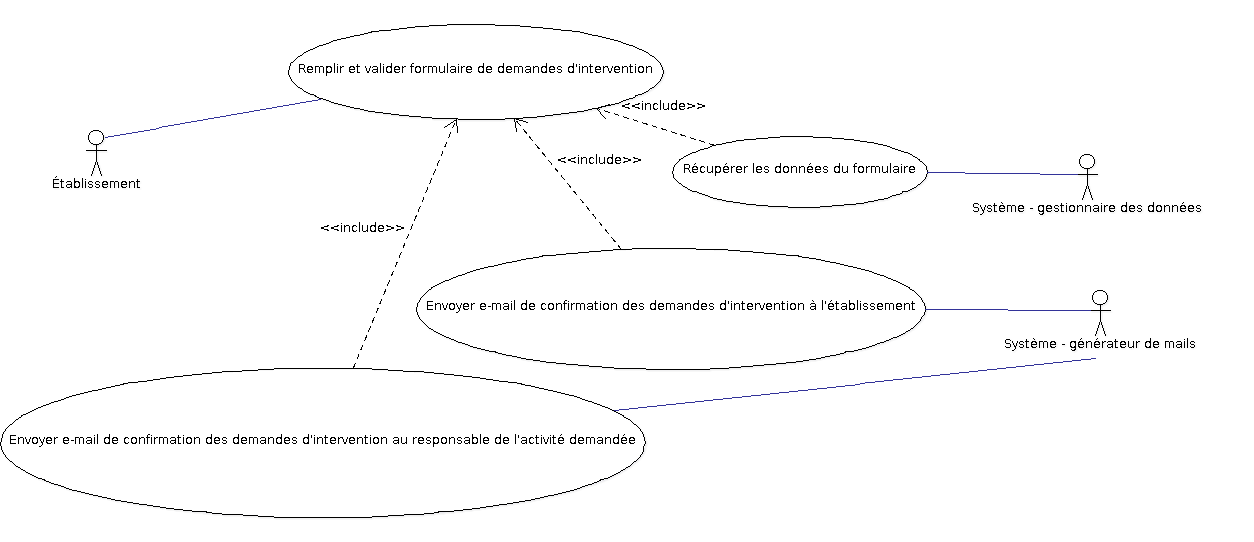
\includegraphics[scale=0.4]{images/casDUtilisation/fonctionnalite4ReceptionIntervention.png}
	 \caption{Cas d'utilisation~: Recevoir la demande d'intervention d'un établissement}
	 \label{recevoirDemandesDIntervention}
\end{figure}

% Figure : version 1.00, date 24/02/16, auteur Michel Cressant
\begin{figure}[H]
	\centering
	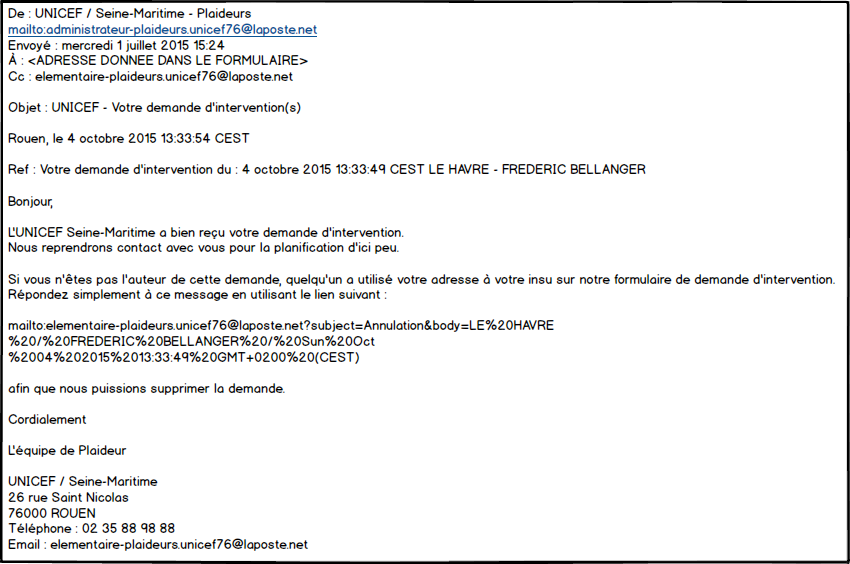
\includegraphics[scale=0.615]{images/maquettes/fonctionnalite4MailConfirmationReceptionDemande.png}
	\caption{Maquette~: Email de confirmation de reception d'une demande d'une école élémentaire}
	\label{maquetteCourrielConfirmation}
\end{figure}

Si un établissement annule une demande d'intervention (grâce à l'e-mail de confirmation d'une demande d'intervention), une procédure supprimera cette demande et enverra des e-mails de confirmation de suppression de cette demande au responsable de l'activité initialement demandée et à l'établissement.Les figures \ref{maquetteCourrielConfirmationAnnulationEtablissement} et {maquetteCourrielConfirmationAnnulationResponsable} présentent une maquette de l'e-mail de confirmation d'annulation pour un établissement et pour un responsable d'activité.\\
  


% Figure : version 1.00, date 24/02/16, auteur Michel Cressant
\begin{figure}[H]
	\centering
	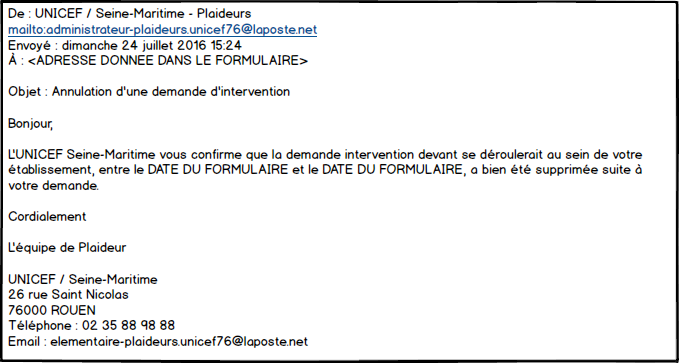
\includegraphics[scale=0.7]{images/maquettes/fonctionnalite4MailConfirmationSuppressionDemandePourEtablissement.png}
	\caption{Maquette~: Email de confirmation d'annulation d'une intervention pour un établissement}
	\label{maquetteCourrielConfirmationAnnulationEtablissement}
\end{figure}

% Figure : version 1.00, date 24/02/16, auteur Michel Cressant
\begin{figure}[H]
	\centering
	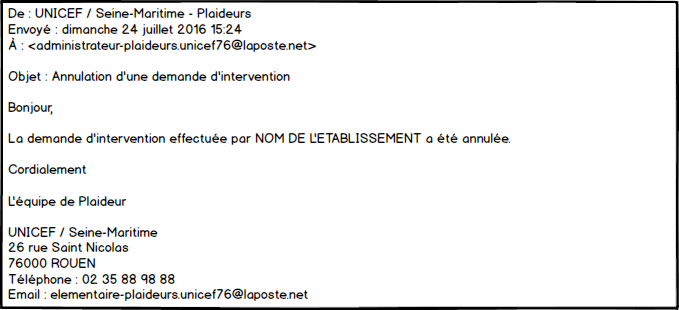
\includegraphics[scale=0.7]{images/maquettes/fonctionnalite4MailConfirmationSuppressionDemandePourAdmin.png}
	\caption{Maquette~: Email de confirmation d'annulation d'une intervention pour le responsable d'activité}	\label{maquetteCourrielConfirmationAnnulationResponsable}
\end{figure}